\subsection{Versionsstyring}
Under udviklingen af spillet er der blevet anvendt git til at versionstyrer udviklingen. Det er blevet lavet et github repository til projektet, samt et til denne rapport.
\newline
Link til spil: \url{https://github.com/Oliver-Olsen/3ugersmatadorExam}
\newline
Link til rapport: \url{https://github.com/joha413/CDIO-Final}

På github kan den nyeste version af spillet og rapporten findes. 
Under udviklingen af spillet er der blevet lavet forskellige forgreninger til at udvikle enkelte funktioner i spillet. "Master" forgreningen, indeholder altid den nyeste version af spillet som virker, mens de andre forgreninger indeholder funktioner der endnu ikke virker, eller er blevet ordentligt testet. 

\subsection{Hent og byg spillet}
Spillet kan fra github hentes og køre. For at gøre dette i Intellij skal man åbne Intellij og trykke på: File \textrightarrow New \textrightarrow Project from Version Control. Derefter kopiere man git repository url ind fra github (figur \ref{fig:git} ). Derefter trykker man Clone

\begin{figure}[h]
    \centering
    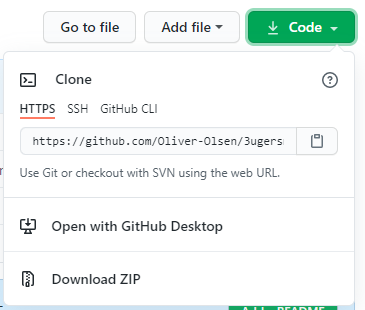
\includegraphics{sources/git.PNG}
    \caption{Github klon værktøj}
    \label{fig:git}
\end{figure}

Når projektet er åbnet i Intellij trykker man på den grønne hammer(eller ctrl+f9) for at bygge projektet.

